% !TEX TS-program = pdflatex
% !TEX encoding = UTF-8 Unicode

% This is a simple template for a LaTeX document using the "article" class.
% See "book", "report", "letter" for other types of document.

\documentclass[20pt]{article} % use larger type; default would be 10pt

\usepackage[utf8]{inputenc} % set input encoding (not needed with XeLaTeX)

%%% Examples of Article customizations
% These packages are optional, depending whether you want the features they provide.
% See the LaTeX Companion or other references for full information.

%%% PAGE DIMENSIONS
\usepackage{geometry} % to change the page dimensions
\geometry{a4paper} % or letterpaper (US) or a5paper or....
% \geometry{margin=2in} % for example, change the margins to 2 inches all round
% \geometry{landscape} % set up the page for landscape
%   read geometry.pdf for detailed page layout information

\usepackage{graphicx} % support the \includegraphics command and options

% \usepackage[parfill]{parskip} % Activate to begin paragraphs with an empty line rather than an indent

%%% PACKAGES
\usepackage{booktabs} % for much better looking tables
\usepackage{array} % for better arrays (eg matrices) in maths
\usepackage{paralist} % very flexible & customisable lists (eg. enumerate/itemize, etc.)
\usepackage{verbatim} % adds environment for commenting out blocks of text & for better verbatim
%\usepackage{subfig} % make it possible to include more than one captioned figure/table in a single float
\usepackage{mathtools}
\usepackage{graphicx} % supports images in latex
% These packages are all incorporated in the memoir class to one degree or another...

\usepackage{graphicx}
\usepackage{subcaption}

%%% Other stuff
\DeclarePairedDelimiter\ceil{\lceil}{\rceil}
\DeclarePairedDelimiter\floor{\lfloor}{\rfloor}

%%% HEADERS & FOOTERS
\usepackage{fancyhdr} % This should be set AFTER setting up the page geometry
\pagestyle{fancy} % options: empty , plain , fancy
\renewcommand{\headrulewidth}{0pt} % customise the layout...
\lhead{}\chead{}\rhead{}
\lfoot{}\cfoot{\thepage}\rfoot{}

%%% SECTION TITLE APPEARANCE
\usepackage{sectsty}
\allsectionsfont{\sffamily\mdseries\upshape} % (See the fntguide.pdf for font help)
% (This matches ConTeXt defaults)

%%% ToC (table of contents) APPEARANCE
\usepackage[nottoc,notlof,notlot]{tocbibind} % Put the bibliography in the ToC
\usepackage[titles,subfigure]{tocloft} % Alter the style of the Table of Contents
\renewcommand{\cftsecfont}{\rmfamily\mdseries\upshape}
\renewcommand{\cftsecpagefont}{\rmfamily\mdseries\upshape} % No bold!

%%% graphics path


%%% END Article customizations

%%% nice things to keep around
%\begin{figure}[!htbp]
%  	\centering
%   	\begin{subfigure}[p]{0.5\linewidth}
%    	\includegraphics[width=\linewidth]{}
%   	\end{subfigure}
%\end{figure} 

% \noindent\rule{2cm}{0.4pt} 
%%% puts a small horizontal line

% \mathcal{O} 
%%% big O notation

% \begin{table}[!htbp]
% \caption{Forward slash.}
% \[\begin{array}{c|ccccc} 
% abc/def & 1 & 2 & 3 & 4 & 5\\
% \hline
% 1 & a & b & c & d & e\\
% 2 & f & g & h & i & j\\
% 3 & k & l & m & n & o\\
% \end{array}\]
% \end{table}

%%% The "real" document content comes below...

\title{Formal Languages Homework 9}
\author{Liam Dillingham}
%\date{} % Activate to display a given date or no date (if empty),
         % otherwise the current date is printed 

\begin{document}
\maketitle

\section{Problem 8.2.1}
\begin{figure}[!htbp]
  	\centering
   	\begin{subfigure}[p]{0.7\linewidth}
    	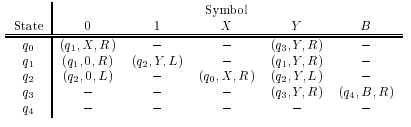
\includegraphics[width=\linewidth]{./figures/HW9fig1.png}
   	\end{subfigure}
\end{figure} 
Show the ID's of the Turning Machine of Fig. 8.9 if the input tape contains:
\subsection{a). 00}
$B q_0 0 0 B \vdash B X q_1 0 B \vdash B X 0 q_1 B$
The machine then halts because the next move is undefined
\subsection{b). 000111}
$B q_0 0 0 0 1 1 1 B \vdash B X q_1 0 0 1 1 1 B \vdash B X 0 q_1 0 1 1 1 B \vdash B X 0 0 q_1 1 1 1 B \vdash B X 0 q_2 0 Y 1 1 B \vdash B X q_2 0 0 Y 1 1 B \vdash B q_2 X 0 0 Y 1 1 B 
\vdash B X q_0 0 0 Y 1 1 B \vdash B X X q_1 0 Y 1 1 B \vdash B X X 0 q_1 Y 1 1 B \vdash B X X 0 Y q_1 1 1 B \vdash B X X 0 q_2 Y Y 1 B \vdash B X X q_2 0 Y Y 1 B \vdash B X q_2 X 0 Y Y 1 B 
\vdash B X X q_0 0 Y Y 1 B \vdash  B X X X q_1 Y Y 1 B \vdash B X X X Y q_1 Y 1 B \vdash B X X X Y Y q_1 1 B \vdash B X X X Y q_2 Y Y B \vdash B X X X q_2 Y Y Y B 
\vdash B X X q_2 X Y Y Y B \vdash B X X X q_0 Y Y Y B \vdash B X X X Y q_3 Y Y B \vdash B X X X Y Y q_3 Y B \vdash B X X X Y Y Y q_3 B \vdash B X X X Y Y Y B q_4 B$
\subsection{c). 00111}
$B q_0 0 0 1 1 1 B \vdash B X q_1 0 1 1 1 B \vdash B X 0 q_1 1 1 1 B \vdash B X q_2 0 Y 1 1 B \vdash B q_2 X 0 Y 1 1 B \vdash B X q_0 Y 1 1 B \vdash B X X q_1 Y 1 1 B \vdash B X X Y q_1 1 1 B \vdash B X X q_2 Y Y 1 B \vdash B X q_2 X Y Y 1 B \vdash B X X q_0 Y Y 1 B \vdash B X X Y q_3 Y 1 B \vdash B X X Y Y q_3 1 B$\\
The machine then halts because the next move is undefined
\newpage
\section{Problem 8.2.2}
Design Turing machines for the following languages:
\subsection{c). $\{ww^{R} \mid w $ is any string of 0's and 1's $\}$}
$$M = ( \{q_0, q_1, q_2, q_3, q_4, q_5, q_f\}, \{0,1\}, \{0,1,B\}, \delta, q_0, B, \{q_f\})$$
\begin{enumerate}
\item $\delta(q_0, 0) = (q_1, B, R)$
\item $\delta(q_0, 1) = (q_f, B, R)$
\item $\delta(q_0, B) = (q_6, B, R)$
\item $\delta(q_1, 0) = (q_1, 0, R)$
\item $\delta(q_1, 1) = (q_1, 1, R)$
\item $\delta(q_1, B) = (q_3, B, L)$
\item $\delta(q_2, 0) = (q_2, 0, R)$
\item $\delta(q_2, 1) = (q_2, 1, R)$
\item $\delta(q_2, B) = (q_4, B, R)$
\item $\delta(q_3, 0) = (q_5, B, L)$
\item $\delta(q_4, 1) = (q_5, B, L)$
\item $\delta(q_5, 0) = (q_5, 0, L)$
\item $\delta(q_5, 1) = (q_5, 1, L)$
\item $\delta(q_5, B) = (q_0, B, R)$
\end{enumerate}
\newpage
\section{Problem 8.2.5}
Consider the Turing Machine
$$M = ( \{q_0, q_1, q_2, q_f\}, \{0,1\}, \{0,1,B\}, \delta, q_0, B, \{q_f\})$$
Informally, but clearly describe the language $L(M)$ if $\delta$ consists of the following set of rules:
\subsection{a). $\delta(q_0, 0) = (q_1, 1, R); \ \delta(q_1, 1) = (q_0, 0, R); \ \delta(q_1, B) = (q_f, B, R)$}
it accepts strings like this: 0101010, that is, strings that start with 0, end with 1, and alternate between 0 and 1 every symbol
\subsection{b). $\delta(q_0, 0) = (q_0, B, R); \ \delta(q_0, 1) = (q_1, B, R); \ \delta(q_1, 1) = (q_1, B, R); \ \delta(q_1, B) = (q_f, B, R)$}
Strings of any length that end with a 1
\subsection{c). $\delta(q_0, 0) = (q_1, 1, R); \ \delta(q_1, 1) = (q_2, 0, L); \ \delta(q_2, 1) = (q_0, 1, R); \ \delta(q_1, B) = (q_f, B, R)$}
Strings that start with a 0, end with a 1, and alternate between 0 and 1
\section{Problem 8.4.2}
Here is the transition function of a nondeterministic $M = (\{q_0, q_1, q_2\}, \{0,1\}, \{0,1,B\}, \delta, q_0, b, \{q_2\})$:
\begin{figure}[!htbp]
  	\centering
   	\begin{subfigure}[p]{0.7\linewidth}
    	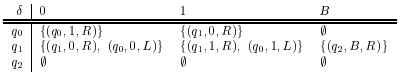
\includegraphics[width=\linewidth]{./figures/HW9fig2.png}
   	\end{subfigure}
\end{figure} 
Show the ID's reachable from the initial ID if the input is:
\subsection{a). 01}
$\{(q_0, 1, R)\} \vdash \{(q_1, 0, r)\} \vdash \{(q_2, B, R)\}$
\subsection{b). 011}
$\{(q_0, 1, R)\} \vdash \{(q_1, 0, r)\} \vdash \{(q_1, 1, R), (q_0, 1, L)\} \vdash \{(q_2, B, R) \} \cup \{(q_0, 1, R)\}$
\end{document}
